\documentclass[reqno]{amsart}

\usepackage[bookmarks=false]{hyperref}
\hypersetup{pdfstartview={XYZ null null 1.50}}
\usepackage{subcaption}
\usepackage{amssymb, amsmath, amsthm, amsfonts,graphicx,relsize,tikz,hyperref,mathtools,esint}
\usetikzlibrary{shapes.geometric,arrows,shapes}
%\usepackage{layout}
\tikzstyle{process} = [rectangle, minimum width=3cm, minimum height=1cm, text centered, draw=black, fill=red!30]
\tikzstyle{decision} = [diamond, minimum width=3cm, minimum height=1cm, text centered, draw=black, fill=green!30]
\tikzstyle{io} = [trapezium, trapezium left angle=70, trapezium right angle=110, minimum width=3cm, minimum height=1cm, text centered, draw=black, fill=blue!30]
\tikzstyle{arrow} = [thick,->,>=stealth]
\tikzstyle{line}=[ draw, -latex']
\textwidth=6in
\textheight=8.75in
\voffset=-.5in
\hoffset=-.5in  %Comment for article
\parindent=20pt   %Comment for article

%\usepackage{color}
\usepackage{xcolor} % needed for urlbordercolor in hyperref
%\usepackage[hyperindex,hypertex,colorlinks=true, linkcolor=blue, urlcolor=blue, citecolor=red, urlbordercolor=blue]{hyperref}

%\usepackage[mathlines,displaymath]{lineno}
%
%%=====
%\newcommand*\patchAmsMathEnvironmentForLineno[1]{%
%  \expandafter\let\csname old#1\expandafter\endcsname\csname
%#1\endcsname
%  \expandafter\let\csname oldend#1\expandafter\endcsname\csname
%end#1\endcsname
%  \renewenvironment{#1}%
%     {\linenomath\csname old#1\endcsname}%
%     {\csname oldend#1\endcsname\endlinenomath}}%
%\newcommand*\patchBothAmsMathEnvironmentsForLineno[1]{%
%  \patchAmsMathEnvironmentForLineno{#1}%
%  \patchAmsMathEnvironmentForLineno{#1*}}%
%\patchBothAmsMathEnvironmentsForLineno{equation}%
%\patchBothAmsMathEnvironmentsForLineno{align}%
%\patchBothAmsMathEnvironmentsForLineno{flalign}%
%\patchBothAmsMathEnvironmentsForLineno{alignat}%
%\patchBothAmsMathEnvironmentsForLineno{gather}%
%\patchBothAmsMathEnvironmentsForLineno{multline}%
%%=====
%
%\linenumbers





%\usepackage{showkeys}
%\usepackage{refcheck} %this is the one you want to use

\usepackage{mathrsfs}
\def\L{{\mathscr L}}
\def\S{{\mathcal S}}
%\def\D{{\mathscr D}}
%\def\I{{\mathscr I}}

\usepackage{array}

%\usepackage[dvips]{color}
%\usepackage{xcolor} % needed for urlbordercolor in hyperref
%\usepackage[pdftex]{hyperref}

\theoremstyle{plain}
\newtheorem{theorem}{Theorem}
\newtheorem{corollary}[theorem]{Corollary}
\newtheorem{lemma}[theorem]{Lemma}
\newtheorem{prop}{Proposition}
\newtheorem{result}{Result}


\theoremstyle{definition}
\newtheorem{definition}{Definition}
\newtheorem{example}{Example}
\newtheorem*{ack}{Acknowledgment}
\newtheorem{remark}[theorem]{Remark}

%\numberwithin{equation}{section}
\numberwithin{theorem}{section}
\numberwithin{definition}{section}
%\numberwithin{lemma}{section}
%\numberwithin{corollary}{section}
\numberwithin{prop}{section}
%\numberwithin{remark}{section}
\numberwithin{example}{section}

%\renewcommand{\H}{\ensuremath{\mathcal{H}}}

\newcommand{\R}{\ensuremath{\mathbb{R}}}
\newcommand{\Z}{\ensuremath{\mathbb{Z}}}
\newcommand{\G}{\ensuremath{\mathbb{H}}}
\newcommand{\N}{\ensuremath{\mathbb{N}}}
\newcommand{\K}{\ensuremath{\mathbb{K}}}
\newcommand{\PT}{\ensuremath{\mathbb{P}}}
\newcommand{\T}{\ensuremath{\mathbb{T}}}
\newcommand{\C}{\ensuremath{\mathbb{C}}}
\newcommand{\I}{\ensuremath{\mathbb{I}}}
\newcommand{\A}{\ensuremath{\mathbb{A}}}
\newcommand{\X}{\ensuremath{\mathbb{X}}}
\newcommand{\D}{\ensuremath{\mathbb{D}}}
\newcommand{\floor}[1]{\lfloor #1 \rfloor}

\newcommand{\Cerg}{\ensuremath{\mathbb{C}_{\text{erg}}}}
\newcommand{\Chilg}{\ensuremath{\mathbb{C}_{\mathcal H}}}
\newcommand{\Rerg}{\ensuremath{R_{\text{erg}}}}
\newcommand{\Ierg}{\ensuremath{I_{\text{erg}}}}


\DeclareMathOperator{\Res}{Res}
\DeclareMathOperator{\myRe}{Re}
\DeclareMathOperator{\myIm}{Im}
\DeclareMathOperator{\rank}{rank}
\DeclareMathOperator{\spec}{spec}
\DeclareMathOperator{\Span}{span}
\DeclareMathOperator{\adj}{adj}
\DeclareMathOperator{\Log}{Log}

\DeclareMathOperator{\Hcos}{Hcos} %Hilger's
\DeclareMathOperator{\Hsin}{Hsin}
\DeclareMathOperator{\Bcos}{Bcos} %Bohner's
\DeclareMathOperator{\Bsin}{Bsin}

\DeclareRobustCommand{\rchi}{{\mathpalette\irchi\relax}}
\newcommand{\irchi}[2]{\raisebox{\depth}{$#1\chi$}} % inner command, used by \rchi

\renewcommand{\Re}{\myRe}
\renewcommand{\Im}{\myIm}
%\def\Re{\textup{\Re\,}}
%\def\Im{\textup{Im\,}}
\def\Reh{{\textup{\Re}_h}}
\def\Imh{{\textup{Im}_h}}
\def\Rem{\myRe_\mu}
\def\Imm{{\textup{Im}_{\mu}}}
%\def\Rem*{{\textup{\Re}_{\mu_*}}}
%\def\Imm*{{\textup{Im}_{\mu_*}}}

\def\ds{\displaystyle}


\newcommand{\s}{\sigma}
\newcommand{\m}{\mu}
\renewcommand{\t}{\tau}
%\newcommand{\D}{\Delta}

%\def\baselinestretch{1.5}\small\normalsize

%\usepackage{ucs}
%\usepackage[utf8x]{inputenc}

\DeclareMathOperator{\ve}{vec}

\usepackage{tikz,amsmath,amssymb}

\usetikzlibrary{patterns}

\DeclareMathOperator{\re}{Re}
\DeclareMathOperator{\im}{Im}
\usetikzlibrary{decorations.pathreplacing,calligraphy}

\def\icirc{\overset{\odot}{\imath}}



\begin{document}

%\pagewiselinenumbers


\title{Generalized Sinusoids and The Time Scale Ergodic Complex Plane}
\author[Poulsen, Davis, Jackson]{Dylan Poulsen$^1$, John M. Davis$^2$, Billy J. Jackson$^3$}
\address{$^1$Department of Mathematics, Washington College, Chestertown, MD 21620-5129}
\email{dpoulsen2@washcoll.edu}
\address{$^2$Department of Mathematics, Baylor University, Waco, TX 76798}
\email{John\_M\_Davis@baylor.edu}
\address{$^3$Department of Mathematics, Statistics, and Computer Science, University of Illinois Chicago, Chicago, IL 60607}
\email{bjjack06@gmail.com}
\keywords{time scales, frequency, power of a point, Hilger complex plane, stability }
\subjclass[2000]{93D05, 93D30, 37B25, 39B42, 15A24}

\begin{abstract}
We introduce a new coordinate system for the complex plane in terms of solutions to the first order linear constant coefficient dynamic equation on time scales. This is an extension of Hilger's complex plane \cite{HiA}, which is based upon an inherently \emph{local} description of the time scale that embraces its \emph{global} structure (making the construction intrinsically ergodic in nature as noted by Jackson and Davis in \cite{JaDaE} and \cite{JaDalap}). We show that the two axes in this coordinate system correspond to exponential growth rate and to frequency. Moreover, we show that in many cases we can think of the change of coordinates as being the result of a conformal map, which leads to interesting geometry when viewed in the complex plane with the standard coordinate system. For example, the boundary of the exponential stability region discovered by Pötzsche et al. \cite{PoSiWi} is one level curve of this conformal map. Finally, with the realizations that sinusoids should have zero exponential growth rate and a distinct frequency, we define a generalization of sine and cosine on time scales distinct from other generalizations in the literature. 
\end{abstract}

\maketitle

%\subsection{Hilger's Complex Plane and Its Relation to Stability and the ROC}

\section{Background}
We begin by offering a brief summary of the Hilger complex plane \cite{BoPeD} on a time scale $\mathbb{T}$. The {\em Hilger real part} of $z \in \C$ at $t \in \mathbb{T}$ is defined as
\begin{eqnarray*}
\text{Re}_{\mu(t)}(z):= \lim_{\tau \to \mu(t)} \frac{|1+\tau z|-1}{\tau},\end{eqnarray*}
while the {\em Hilger imaginary part} of $z$ is given by
\begin{equation}
\label{eq:HilgerImagPart}
    \text{Im}_{\mu(t)}(z):= \lim_{\tau \to \mu(t)}\frac{\text{Arg}(z\tau+1)}{\tau},
\end{equation}
where the argument is the principal argument satisfying $-\pi < \text{Arg} (z) \leq \pi$.  The {\em purely imaginary Hilger number} is given by
$$ \stackrel{o}{\iota} \omega:= \lim_{\tau \to \mu(t)}\frac{e^{i\omega \tau}-1}{\tau}.$$ The {\em circle plus operation} $\oplus$ is defined by $a \oplus b=a+b+\mu(t) ab$, and using this, every $z \neq -\frac{1}{\mu(t)}$ can be written as $$z=\text{Re}_{\mu(t)}(z) \oplus  \stackrel{o}{\iota}  \text{Im}_{\mu(t)}(z).$$
The {\em circle minus operation} $\ominus$ is defined to be the inverse of $\oplus$. See \cite{BoPe} for a complete treatment. Hilger's decomposition of the complex plane is shown in Figure~\ref{fig:complexplane}.

\begin{figure}
\centering
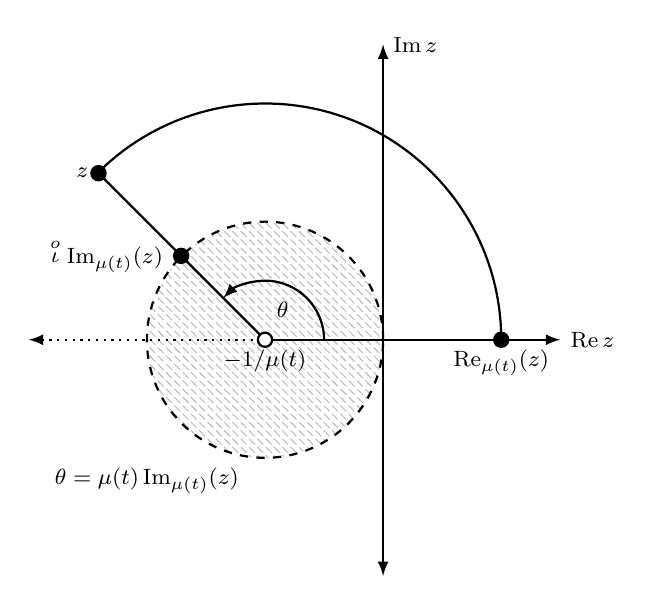
\begin{tikzpicture}[scale=1.5]
    \tikzset{>=latex}
    \begin{scope}[thick,font=\footnotesize]
    \filldraw[pattern=north west lines, pattern color=lightgray,dashed] (-1,0) circle (1);

    \draw [->] (-1,0) -- (1.5,0) node [right]  {Re$\,z$};
    \draw [<-,dotted] (-3,0) -- (-1,0);
    \draw [<->] (0,-2) -- (0,2.5) node [right] {Im$\,z$};
    %\draw [-] (-1,0) -- (-2.41,1.41) node [right] {$z$};
    \draw [-] (-1,0) -- (-2.41,1.41) node [left] {$z$};
    \draw[->] (-.5,0) arc (0:135:.5cm);
    \draw[-] (1,0) arc (0:135:2cm);

    \node at (-.85,.25) {$\theta$};
    \node at (1,0) [below] {$\re_{\mu(t)}(z)$};
    \node at (-1.71,.71) [left,xshift=-.1cm] {$\stackrel{o}{\iota} \im_{\mu(t)} (z)$};

    \filldraw[fill=black, draw=black] (-1.71,.71) circle (.06);
    %\filldraw[fill=black, draw=black] (-2.41,1.41) circle (.06);
    \filldraw[fill=black, draw=black] (-2.41,1.41) circle (.06);
    \filldraw[fill=black, draw=black] (1,0) circle (.06);

    %\draw (-1,-3pt) -- (-1,3pt) node [below,yshift=-0.2cm] {$-1/\mu$};

    \node at (-1,0) [below,yshift=-0.0cm] {$-1/\mu(t)$};
    \node at (-2,-1) [below,yshift=-0.0cm] {$\theta=\mu(t) \im_{\mu(t)}(z)$};

    \filldraw[fill=white, draw=black] (-1,0) circle (.06);

    \end{scope}
\end{tikzpicture}
\caption{Hilger's Complex Plane, $\Chilg$. Numbers $z$ inside the circle have negative Hilger real part, while points on the circle have zero Hilger real part. Numbers $z$ outside the circle have positive Hilger real part.}
\label{fig:complexplane}
\end{figure}

Some possible notations:

Hilger complex plane $\mathbb{C}_{\mathcal H}$

Ergodic complex plane $\Cerg$

Hilger ``circle" at $t$ (so corresponding to $\mu(t)$): $\mathcal{H}_t$ or $\mathcal{H}_{\mu(t)}$
a.k.a. Hilger imaginary disk $\mathcal{H}_t$

Hilger *circle* $\partial\mathcal{H}_t$ or $\partial\mathcal{H}_{\mu(t)}$

In \cite{JaDaPo}, we've shown that Hilger's representation can actually be considered as a type of polar form for time scales.  One goal of this work is to show how this polar perspective offers significant geometric insight and explanation to various concepts in the time scales literature.  

\section{Polar Geometry}
From a polar standpoint, Hilger's definitions can be visualized as in Figure~\ref{fig:hilgerpolar}.  The Hilger real part of $z \in \C$ can be thought of as the power of $z$ with respect to the Hilger imaginary disk; points exterior to the disk have positive power, points on the disk have zero power, and points interior to the disk have negative power.  From this vantage point, Hilger's definitions induce a tangential metric for the complex plane for $z$ having Hilger real part  $R_\mu$ and for a fixed $\mu$, via $$d(z,\G_\mu)=\sqrt{\left|R_\mu^2+\frac{2}{\mu}R_\mu\right|}.$$ (NEED TO INCLUDE $\G_\mu$ DEF.)

\begin{figure}
\centering
\begin{tabular}{cc}
\begin{subfigure}{.5\textwidth}\centering\includegraphics[width=\columnwidth]{images/hilgercomplexplanetangents.jpg}\caption{$\text{Re}_\mu(z)>0$}\label{fig:hilrealpos}\end{subfigure}&
\begin{subfigure}{.5\textwidth}\centering\includegraphics[width=\columnwidth]{images/hilrepartneg.jpg}\caption{$\text{Re}_\mu(z)<0$}\label{fig:hilrealneg}\end{subfigure}\\
\newline
\begin{subfigure}{.5\textwidth}\centering\includegraphics[width=\columnwidth]{images/polarmuzerosmaller.jpg} \caption{$\text{Re}_{\mu_1}(z)>0$}\label{fig:hilzerosmall}\end{subfigure}&
\begin{subfigure}{.5\textwidth}\centering\includegraphics[width=\columnwidth]{images/polarmuzerolarger.jpg} \caption{$\text{Re}_{\mu_2}(z)>0, \mu_2<\mu_1$}\label{fig:hilzerolarge}\end{subfigure} \\
%\includegraphics[scale=0.125]{images/hilgerpolarzero.jpg} 
\end{tabular}
\caption{The Hilger real part is illustrated in various cases.  Hilger's formalism determines a tangential metric for points in the complex plane, as shown.  The bottom row shows how $\text{Re}_\mu(z)\to \text{Re}(z)$ as $\mu \to 0$.}
\label{fig:hilgerpolar}
\end{figure}

Notice as we see in Figure~\ref{fig:hilgerpolar}, $\G_\mu$ tends to the imaginary axis as $\mu \to 0$, or from Hilger's perspective, the imaginary axis is the boundary of an disk with infinite radius tangent to the origin.  For $z$ exterior to $\G_\mu$ and $\mu=0$ in the limit (i.e., so that $z$ lies in the right half plane), $Re(z)$ is the length of the line segment that extends from the boundary of the disk to $z$ itself: this line segment lies on the line passing through the center of the disk and $z$. Put another way, in terms of the metric, the distance from $z$ to the imaginary Hilger disk is simply $Re(z)$.  For $z$ in the left half plane (and thus interior to the infinite Hilger imaginary disk in the limit), the tangent line to the inner disk $\text{Re}_\mu(w)=\text{Re}_\mu(z)$ tends to the vertical position meaning that the distance between the two disks obtained in the limit is $-\text{Re}_\mu(z)$.  Thus, $R_{\mu}(z) \to \text{Re}(z)$ in both cases, as expected.

The sign of the Hilger real part of $z$ is determined by its relation to the {\em Hilger imaginary disk}. The $\stackrel{o}{\iota}$ operator parameterizes the boundary of the Hilger imaginary disk in terms of the frequency $\omega$. If $\mu(t)>0$, the $\stackrel{o}{\iota}$ operator is a bijection if we restrict the domain of the operator to $(-\pi/\mu(t),\pi/\mu(t)]$. Points on the boundary of the disk have zero Hilger real part, while points interior have negative Hilger real part and points exterior have positive Hilger real part. The sign of the Hilger real part determines the {\em local} growth rate of the time scales exponential function at time $t \in \mathbb{T}$. Since the Hilger complex plane changes for each value $t \in \mathbb{T}$, the global dynamics of the time scales exponential function can be inferred from the Hilger complex plane if and only if the time scale is of the form $\mathbb{T}=h \mathbb{Z}$. In this case, the Hilger real part corresponds to the ergodic real part.

The value of the Hilger imaginary part of $z$ is determined by measuring the angle $\theta$ from the center of the Hilger imaginary disc to the point $z$, then dividing by $\mu(t)$. If $\mu(t)=0$, then \eqref{eq:HilgerImagPart} implies that the Hilger imaginary part corresponds exactly to the usual imaginary part of $z$. For time scales of the form $\mathbb{T}=h \mathbb{Z}$, Hilger showed that the Hilger imaginary part corresponds to frequency in the interval $(-\pi/h,\pi/h]$. Note that this is exactly the Nyquist interval for uniform sampling with rate $h$. It is difficult to give a local interpretation of frequency, which perhaps helps to explain why the idea of frequency on time scales has received much less attention than the exponential growth rate.

Discrete: dont think of as radius and angle but rather contours of equal exponential growth rate (radius) and contours of equal frequency (angle)


More generally: $\Cerg$ decomposes $C$ into contours where $\Rerg=c_1$ and $\Ierg=c_2$.

NOTE: Hilger complex plane has these twin contours: exponential growth contour and frequency contour, i.e. the contour where Hilger real part is constant vs. the contour where the Hilger imaginary part is constant

Given a time scale, BoPe showed us how to construct an exponential function on that time scale. EVERY exponential function has two numbers that go with it---exp growth rate and frequency. Can do this on Z (will get regualr polar). Can do this on R (will get rectangular). Can do this on T (with Hilger's viewpoint). Now can do this on T with our viewpoint.

\section{History and Notation of Time Scales Sinusoids}
It is worth examining the history of sinusoids on time scales. Hilger \cite{Hilger1999} defined the cosine and sine functions of frequency $\omega$ on time scales by 
\begin{subequations}
\begin{align}
\Hcos_{\omega}(t,t_0) &:= {e_{\stackrel{o}{\iota} \omega}(t,t_0)+ e_{\ominus \stackrel{o}{\iota} \omega}(t,t_0)\over 2}=\cos(\omega (t-t_0)),\label{eq:hilger_cos}\\
\Hsin_{\omega}(t,t_0) &:= {e_{\stackrel{o}{\iota} \omega}(t,t_0)- e_{\ominus \stackrel{o}{\iota} \omega}(t,t_0)\over 2i}=\sin(\omega (t-t_0)).\label{eq:hilger_sin}
\end{align}\label{eq:hilger}
\end{subequations}
By using the $\stackrel{o}{\iota}$ operator, Hilger defined the cosine function in terms of the exponential function evaluated at points on the boundary of the Hilger imaginary disk; thus, the domain of the $\Hcos_{\omega}$ as a function of $\omega$ is the boundary of the Hilger imaginary disk. This ensures that $\Hcos_{\omega}$ has a zero exponential growth rate in $t$ when $\mathbb{T} = h \mathbb{Z}$.

Hilger went on to show that for time scales of the form $\mathbb{T}=h \mathbb{Z}$, the Hilger imaginary part corresponds to frequency, and that $\Hcos_{\omega}(t,t_0)$ interpolates the real-valued function $\cos(\omega t).$ This property can be referred to as {\it exact discretization} \cite{Cielinski} or {\it perfect interpolation}. Hilger's definitions \eqref{eq:hilger} are tied to the local aspect of the Hilger complex plane, in the sense that the sinusoids only have the desired global properties of zero growth rate and fixed frequency when the local behavior is the same as the global behavior; that is, $\mu(t)$ is constant for all $t \in \mathbb{T}$, i.e., $\mathbb{T}=h\mathbb{Z}$. 

In general, Hilger's sinusoids have a fixed amplitude of 1 and fixed frequency of $\omega$.  The subscripts are time varying and as such can be thought of as dynamic eigenvalue (pole) placement to ensure that the sinusoids stay bounded and oscillate over time. Since the poles are complex conjugates and the Hilger circle is symmetric with respect to the real axis, a linear combination of exponential functions with complex conjugate subscripts will ensure the sinusoids are real valued again while also remaining bounded in each individual subscript which lies on the Hilger circle. As the pole placement is dynamic, Hilger's sinusoids have derivatives that depend explicitly on $\mu$ and are therefore in some sense dependent on local beahvior of the time scale.  Indeed, we have:
\begin{eqnarray*}
\Hcos_{\omega}^{\Delta}(t,t_0) &= & \lim_{s\to \mu(t)}\frac{\cos (\omega (t-t_0))(\cos (\omega(s-t_0))-1) -\sin(\omega(t-t_0))\sin(\omega(s-t_0))}{s} \\
\Hsin_{\omega}^{\Delta}(t,t_0) & = & \lim_{s\to \mu(t)}\frac{\sin (\omega (t-t_0))(\cos (\omega(s-t_0))-1) +\cos(\omega(t-t_0))\sin(\omega(s-t_0))}{s}
\end{eqnarray*}
This means that Hilger's sinusoids have dynamic pole placement that results in a dynamic calculus in the sense that his sinusoids have derivatives that vary as the time scale $\T$ changes.  However, it also true that on periodic time scales, his sinusoids will be periodic for those frequencies that are proportional to $\pi$, with the proportionality constant depending upon the period of the time scale in general.

By comparison, Bohner and Peterson \cite{BoPeD} chose a different generalization of the sinusoids, defining the time scale cosine and sine functions of frequency $\omega$ as
\begin{subequations}
\begin{align}
\Bcos_{\omega}(t,t_0) &:= {e_{i \omega}(t,t_0) + e_{-i \omega}(t,t_0) \over 2},\label{eq:bope_cos}\\
\Bsin_{\omega}(t,t_0) &:= {e_{i \omega}(t,t_0) - e_{-i \omega}(t,t_0) \over 2i}.\label{eq:bope_sin}
\end{align}\label{eq:bope}
\end{subequations}
Using the time scale polar form from \cite{JaDaPo}, for $R_\mu=\text{Re}_{\mu}(i \omega)$, $I_\mu=\text{Im}_{\mu}(i \omega)$ and $\theta_\mu=\mu I_\mu$, it follows that on purely discrete time scales
\begin{eqnarray}
B\cos_\omega(\sigma(t),t_0) &= & \text{Re}\left(e_{i \omega}(t,t_0)\right) \notag\\
& = & \text{Re} \left(\prod_{s=t_0}^{t} (1+\mu(s) i \omega) \right) \notag \\
& = & \text{Re} \left ( \prod_{s=t_0}^t \left(1+\mu(s) \left(\left(R_\mu+\frac{1}{\mu(s)}\right)e^{i \theta_\mu}-\frac{1}{\mu(s)}\right)\right)\right) \notag \\
& = & \text{Re} \left( \prod_{s=t_0}^{t} (1+\mu(s) R_\mu) \cdot e^{\sum_{s=t_0}^{t} i \theta_\mu}\right) \notag \\
& = & \prod_{s=t_0}^{t} |1+ \mu(s) i \omega| \cdot \cos\left(\sum_{s=t_0}^{t}  \theta_\mu}\right) \label{bpcospol}
\end{eqnarray}
Likewise,
\begin{eqnarray}
B\sin_\omega(t,t_0) & = & \text{Im} \left( e_{ i \omega}(t,t_0)\right) \notag \\
& = & \prod_{s=t_0}^{t} |1+ \mu(s) i \omega| \cdot \sin\left(\sum_{s=t_0}^{t}  \theta_\mu}\right) \label{bpsinpol}
\end{eqnarray}
From (\ref{bpcospol}) and (\ref{bpsinpol}), we see that the Bohner and Peterson sinusoids are oscillatory in general as $\sum_{s=t_0}^{t}  \theta_\mu}\right)$ cycles through the four quadrants as $t \in \T$ changes. These sinsuoids will not be periodic for any frequency in general even for periodic time scales as the amplitude grows without bound for all nonzero $\omega$, and as follows from \cite{PoSiWi}, neither will they be bounded even on $h \Z$. As seen from (\ref{bpcospol}) and (\ref{bpsinpol}), Bohner and Peterson's sinusoids have time varying amplitudes and frequencies.  

However, in terms of calculus, the Bohner and Peterson definitions have dynamic advantages, in the sense that the derivative of $\Bcos_{\omega}$ is proportional to $\Bsin_{\omega}$, and vice-versa:
\begin{eqnarray}
    B\cos_\omega^{\Delta}(t,t_0) & = & -\omega B\sin_{\omega}(t,t_0) \label{bpcosder}\\
    B\sin_\omega^{\Delta}(t,t_0) & = & \omega B\cos_{\omega}(t,t_0) \label{bpsinder}
\end{eqnarray}

Thus, in contrast to Hilger's sinusuoids, the Bohner and Peterson sinusoids have derivatives that are independent of $\mu$ (at least explicitly) and thus are not tied to the local nature of the time scale near $t$.  Therefore their sinusuoids have static pole placement as the subscripts are time independent and their calculus is also static in the sense that the derivatives are identical on all time scales as is seen in (\ref{bpcosder}) and (\ref{bpsinder}).
By formulating the time scale exponential in terms of $i \omega$ rather than $\stackrel{o}{\iota}\omega$, the domain of $\Bcos_{\omega}$ (as a function of $\omega$) is not restricted to the boundary of the Hilger imaginary disk and thus the pole placement is static . Thus, in general, $\Bcos_{\omega}$ is not bounded in $t$. This is a fundamental difference in the formulations \eqref{eq:hilger} and \eqref{eq:bope} and will be a recurring theme in this paper.

Unification and extension are two dominant yet opposing themes in the theory of dynamic equations on time scales. In some sense, $\Hcos_{\omega}$ successfully unifies the cosine function on $\mathbb{R}$ and $h\mathbb{Z}$, but it does not extend the perfect interpolation beyond these cases. On the other hand, $\Bcos_{\omega}$ extends the cosine based on its dynamic properties, but sacrifices the unifying property of boundedness. 

There have been numerous other attempts to generalize time scale sinusoids. For example, Bohner and Peterson \cite{BoPe} also give a completely separate derivation of the so-called alternate trigonometric functions \cite{BoPe, Sec. 3.6}. On the other hand, Mesquita {\it al} \cite{} used a Laplace transform approach to derive their time scale sine and cosine functions and used them to analyze second-order Cauchy problems.

Our methods here are an amalgamation of Hilger's and Bohner and Peterson's approaches: we take the view that the time scale sine and cosine should have zero exponential growth rate and should have a well-defined frequency within the Nyquist interval for the time scale, just as $\Hcos_{\omega}(t,t_0)$ does when $\mathbb{T}=h\mathbb{Z}$. The generalized time scale functions should also exhibit the ``nice" calculus properties of the Bohner and Peterson sinusoids. Since these properties follow from the construction of the Hilger complex plane and the accompanying forms of the subscripts in the complex exponentials, we accomplish our generalization of time scale sinusoids by generalizing the Hilger complex plane from the {\em local} properties of $\T$ to its {\em global} properties.

To accomplish this, we need to expand the Hilger complex plane to show not just the Hilger imaginary disc (which corresponds to a contour where the exponential growth rate is zero), but to show the contours of equal exponential growth rate. It is also helpful to show the contours of equal frequency (i.e., Hilger imaginary part). See Figure \ref{fig:h_limit}.

%graphics from Ergodic COmplex Plane.nb
{\centering
\begin{figure}
\begin{tabular}{ccc}
\begin{subfigure}{0.33\textwidth}\centering\includegraphics[width=\columnwidth]{images/lim_1.png}\caption{$h=1$}\label{fig:h_1}\end{subfigure}&
\begin{subfigure}{0.33\textwidth}\centering\includegraphics[width=\columnwidth]{images/lim_1_2.png}\caption{$h=1/2$}\label{fig:h_2}\end{subfigure}&
\begin{subfigure}{0.33\textwidth}\centering\includegraphics[width=\columnwidth]{images/lim_1_4.png}\caption{$h=1/4$}\label{fig:h_4}\end{subfigure}\\
\newline
\begin{subfigure}{0.33\textwidth}\centering\includegraphics[width=\columnwidth]{images/lim_1_8.png}\caption{$h=1/8$}\label{fig:h_8}\end{subfigure}&
\begin{subfigure}{0.33\textwidth}\centering\includegraphics[width=\columnwidth]{images/lim_1_16.png}\caption{$h=1/16$}\label{fig:h_16}\end{subfigure}&
\begin{subfigure}{0.33\textwidth}\centering\includegraphics[width=\columnwidth]{images/lim_1_32.png}\caption{$h=1/32$}\label{fig:h_32}\end{subfigure}\\
\end{tabular}
\caption{The contours of equal exponential growth rate (dotted) and of equal frequency (dashed) of the time scales exponential function on $\mathbb{T} = h \mathbb{Z}$ for various values of $h$. The contour with zero exponential growth rate (which corresponds to the Hilger imaginary disk) is solid. As $h\to 0^+$, the contours morph from defining a shifted polar coordinate system to a rectangular coordinate system.}
\label{fig:h_limit}
\end{figure}
}

As we can see, the contours of equal exponential growth rate are perpendicular to the contours of equal frequency. In fact, the exponential growth rate and the frequency have induced a (shifted) polar coordinate system on the complex plane. We have investigated the usefulness of this polar form in \cite{JaDaPo} and in fact used contours of equal exponential growth rate \emph{plus} $1/\mu(t)$ instead of just contours of equal exponential growth rate.

Note also in the limit as $h \rightarrow 0^{+}$, the center of the circles approaches negative infinity, and the contours of equal exponential growth rate and of equal frequency become grid lines in the usual rectangular coordinates. This coincides with the case $\mathbb{T}=\mathbb{R}$, where $e_{z}(t,t_0) = e^{z(t-t_0)}$, and the exponential growth rate is given by $\Re(z)$ while the frequency is given by $\Im(z)$.

\section{The Time Scale Ergodic Complex Plane}

FRAMING THE NARRATIVE: Goal is to do Fourier analysis of arb signals on arb time scales

Let's understand the domain frequency divorced from the signal frequency. We will see that the domain frequency induces a geometry on the complex plane that naturally defines the  frequency of the signal itself.

Inherent: time scale itself has a frequency or timing associated with it. But then a signal on the time scale has its own frequency or timing associated with it. These are distinct notions of {\it frequency} which interact with one another throughout this work.

$\T_{1,2}$ versus the (modified) Thue-Morse sequence... T-M is nonperiodic, yet has equal weights of 1's and 2's and yet is asymptotically equivalent to $\T_{1,2}$

Note there is a timing inherent from the time scale itself. But if we analyze a signal on either of these time scales, the signal will have its own notion of {\it frequency} or {\it sampling} or {\it timing}.





Hilger's complex plane is an effective tool to analyze the behavior of the time scale exponential function {\em locally} (that is, at a fixed $t \in \mathbb{T}$). For example, if $\lambda$ is inside (outside) the Hilger imaginary disk at time $t$, then $|e_{\lambda}(t,t_0)|$ is decreasing (increasing) at time $t$. The Hilger imaginary disk is therefore a {\em dynamic} region of stability for the time scale exponential. In 2003, P\"{o}tzsche {\it et al.} \cite{PoSiWi} found a necessary and sufficient condition on $\lambda$ to guarantee that $e_{\lambda}(t,t_0)$ approaches zero at an exponential rate as $t\to \infty$; that is, they found a {\em static} region of stability. To summarize, a change in perspective was made from {\em local} and {\em dynamic} to {\em global} and {\em static}. 

(JOHN, THIS COULD USE EXPANSION) Jackson and Davis \cite{??} later discovered that the condition of P\"{o}tzsche {\it et al.} was in some sense an average of the Hilger real part, and that the static region of stability was in some sense the average of Hilger imaginary disks at every time in the time scale. Poulsen \cite{??} used this observation to develop the stability theory for stochastically generated time scales, where the graininess is a random variable. In this setting, the averaging of the Hilger real parts was even more clear. 

DO WE INCLUDE THE PSW THEOREM, ESPECIALLY IN LIGHT OF THE COMING DEFINITION?

While averaging the Hilger real part has a clear meaning in terms of the global {\it exponential decay rate} of the time scale exponential function,  (NOTE TO SELF/JOHN, WE NEED TO EMPHASIZE THE HILGER REAL PART AS A LOCAL DECAY/GROWTH RATE), to our knowledge no one has examined the meaning of averaging the Hilger imaginary part. Since on $h \mathbb{Z}$, the Hilger imaginary part corresponds to a unique frequency in the interval $(-\pi/h,\pi/h],$ it stands to reason that the average of the Hilger imaginary parts represents a sort of global {\it frequency} of the time scale exponential function. To investigate this further, we need some definitions.

\begin{definition}
Let $\mathbb{T}$ be an unbounded time scale. Suppose $x,y \in \mathbb{R},$ and let $\lambda := x+iy$, where $\lambda$ is regressive. The {\em ergodic real part} of $\lambda$ is given by
$$\Rerg(x,y)=\limsup_{T \rightarrow \infty} {1\over T-t_0}\int_{t_0}^{T} \lim_{s \rightarrow \mu(t)^{-}} \frac{\ln |1+(x+iy)s|}{s} \Delta s.$$ 
The {\em ergodic imaginary part} of $\lambda$ is given by
$$\Ierg(x,y) = \limsup_{T \rightarrow \infty}  {1\over T-t_0}\int_{t_0}^{T} \lim_{s \rightarrow \mu(t)^{-}} \frac{\text{Arg}(1+(x+iy)s)}{s} \Delta s}.$$
\end{definition}

\begin{definition}
Let $\mathbb{T}$ be periodic and let $\{\mu_k\}_{k\in\Omega}$ be the set of at most countably many graininesses in one period. The {\em ergodic complex plane} $\Cerg$ associated with $\mathbb T$ is defined as $\Cerg:=\mathbb{C}\setminus\{-1/\mu_k\}_{k \in \Omega}$. 
\end{definition}

\begin{example}
Suppose $\mathbb{T}=\mathbb{T}_{1,2},$ the discrete periodic time scale generated by the set $\{1,2\}$. The contours of $\Rerg(x,y)$ and $\Ierg(x,y)$ in $\Cerg$ are shown in the left image of Figure \ref{fig:T2_ECP}.
\end{example}
\begin{example}
Suppose $\mathbb{T}=\mathbb{T}_{2,13},$ the discrete periodic time scale generated by the set $\{2,13\}$. The contours of $\Rerg(x,y)$ and $\Ierg(x,y)$ in $\Cerg$ are shown in the right image of Figure \ref{fig:T2_ECP}. In particular, the boundary of the region of exponential stability on $\mathbb{T}_{2,13}$ is disconnected.
\end{example}
\begin{figure}
    \centering
    \includegraphics[width=.45\columnwidth] {images/T12_ECP.png}
    \includegraphics[width=.45\columnwidth] {images/T213_ECP.png}
    \caption{Contours of $R_{\text{erg}}(x,y)$ (dotted) and $\Ierg(x,y)$ (dashed) in $\Cerg$ for two time scales. The contour with zero exponential growth rate (which corresponds to the boundary of the region of exponential stability) is solid. Left: $\mathbb{T}=\mathbb{T}_{1,2}.$ Right: $\mathbb{T}=\mathbb{T}_{2,13}.$}
    \label{fig:T2_ECP}
\end{figure}
The contours of equal ergodic real part in both images in \ref{fig:T2_ECP} are examples of Cassini ovals, which leads to an interesting physical interpretation. If two infinitely long, parallel wires were carrying equal currents in the same direction, then the magnetic field lines in any plane perpendicular to the wires would match the contours of equal ergodic real part in Figure \ref{fig:T2_ECP} if the wires went through the points of non-regressivity. Similarly, the contours of equal ergodic imaginary part would match the electrostatic field lines, and are examples of rectangular hyperbolas. A similar physical interpretation for more complicated time scales can also be achieved using Cassini curves (SOURCE: https://mathcurve.com/courbes2d.gb/orthogonale/orthogonale.shtml)

\begin{example}
Suppose $\mathbb{T}=P_{a,b}$, the pulse time scale with a repeated pattern of an interval of length $a$ followed by a gap of length $b$. The contours of $\Rerg(x,y)$ and $\Ierg(x,y)$ in $\Cerg$ are shown in the left image of Figure \ref{fig:P2_ECP} for $a=1/4, b=1$. 
\end{example}
\begin{example}
Suppose $\mathbb{T}=C_{1/3}$, which is the time scale consisting of repeated middle-third Cantor sets. The contours of $\Rerg(x,y)$ and $\Ierg(x,y)$ in $\Cerg$ are shown in the right image of Figure \ref{fig:P2_ECP}. 
\end{example}
\begin{figure}
    \centering
    \includegraphics[width=.45\columnwidth] {images/Pab_ECP.png}
    \includegraphics[width=.45\columnwidth] {images/C_ECP.png}
    \caption{Contours of $\Rerg(x,y)$ (dotted) and $\Ierg(x,y)$ (dashed) in $\Cerg$ for two time scales. The contour with zero exponential growth rate (which corresponds to the boundary of the region of exponential stability) is solid. Left: $\mathbb{T}=P_{1/4,1}$ Right: $\mathbb{T}=C_{1/3}.$}
    \label{fig:P2_ECP}
\end{figure}


\begin{lemma}
\label{lem:analytic}
Let $\mathbb{T}$ be an unbounded time scale. Suppose $x,y \in \mathbb{R},$ and let $\lambda := x+iy$, where $\lambda$ is regressive. Define $$f(\lambda) = \limsup_{T \rightarrow \infty} \frac{\Log(e_{\lambda}(T,t_0))}{T-t_0},$$ where $\Log$ denotes the principal logarithm. Then
\begin{enumerate}
    \item $f(\lambda) = \Rerg(x,y) + i \Ierg(x,y).$
    \item Under the additional assumption that $\mathbb{T}$ is periodic, $f$ is analytic and one-to-one on $\Cerg$.
\end{enumerate} 
\end{lemma}
\begin{proof}
For (1), note that
\begin{align*}
f(\lambda) & = \limsup_{T \rightarrow \infty} \frac{\Log(e_{\lambda}(T,t_0))}{T-t_0} \\
        & = \limsup_{T \rightarrow \infty} {1\over T-t_0} \int_{t_0}^{T} \lim_{s \rightarrow \mu(t)^{-}} \frac{\Log (1+(x+iy)s)}{s} \Delta s \\
& = \limsup_{T \rightarrow \infty} {1\over T-t_0}\int_{t_0}^{T} \lim_{s \rightarrow \mu(t)^{-}} \frac{\ln|1+(x+iy)s| + i \text{Arg}(1+(x+iy)s)}{s} \Delta s \\
& = \limsup_{T \rightarrow \infty} {1\over T-t_0}\left(\int_{t_0}^{T} \lim_{s \rightarrow \mu(t)^{-}} \frac{\ln|1+(x+iy)s|}{s} \Delta s +  i \int_{t_0}^{T} \lim_{s \rightarrow \mu(t)^{-}}\frac{\text{Arg}(1+(x+iy)s)}{s} \Delta s\right) \\
& = \Rerg(x,y)+i\Ierg(x,y).
\end{align*}

For (2), when $\mathbb{T}$ is periodic, then there is a number $p$ such that if $t_0 \in \mathbb{T}$, then $t_0 +p \in \mathbb{T}.$ In this case,
$$
f(\lambda) = \frac{\Log(e_{\lambda}(t_0+p,t_0)}{p}.
$$
Since the principal logarithm is analytic and $e_{\lambda}$ is analytic for regressive $\lambda$ (CITE), it follows that $f$ is analytic. Moreover, since the principal Logarithm is one-to-one, and by uniqueness of solutions to first order dynamic equations, $e_{\lambda}(t_0+p,t_0)$ is a one-to-one function of $\lambda$ for regressive $\lambda$, it follows that $f$ is one-to-one.
\end{proof}

Since $f$ is analytic, it is a conformal mapping, so we have the following.
\begin{corollary}
Suppose $\mathbb{T}$ is periodic. The contours of equal ergodic real part and of equal ergodic imaginary part are orthogonal for every point in $\Cerg$.
\end{corollary}

\begin{theorem}
Let $\mathbb{T}$ be a purely discrete periodic time scale generated by the sequence $\{\mu_1,\mu_2,\ldots,\mu_n\}$ (WE'LL NEED TO DEFINE THIS). Define 
$$ a := {1\over n}\sum_{k=1}^{n} \mu_k = {1\over n}\int_{t_0}^{t_n} \Delta t = \frac{t_n-t_0}{n}.$$
\begin{enumerate}
    \item The contour of zero ergodic real part is bounded.
    \item The range of the ergodic imaginary part is $(-\pi/a,\pi/a].$ 
\end{enumerate}
\end{theorem}
\begin{proof}
SKETCH: the proof of (1) relies on the fact that the PSW region lies within the largest Hilger Circle (smallest graininess). Should be a fairly straightforward inequality.

The proof of (2) relies on the symmetry of the frequency contours and the fact that we know the angle in every Hilger complex plane for the leftmost point on the boundary of the stability region. Essentially, we're averaging an argument, but that argument should be the same for every point at the leftmost point on the boundary of the stability region.
\end{proof}

\begin{remark}
    If $\mathbb{T}$ is a purely discrete periodic time scale generated by the sequence of graininesses $\{\mu_1,\mu_2,\ldots,\mu_n\}$, and if $t \in \mathbb{T}$ is measured in seconds, then we have the following.
    \begin{enumerate}
        \item The average sampling rate is $1/a$ samples per second.
        \item The Nyquist-Shannon sampling theorem implies that we can perfectly reconstruct a continuous time signal sampled on the time scale that contains no frequencies higher than $\frac{1}{2a}$ hertz. That is, we can perfectly reconstruct a continuous time signal sampled on the time scale that contains no frequencies higher than $\pi/a$, which is exactly the bound on the magnitude of the range of ergodic imaginary part.
        \item Thus, the definition of the ergodic imaginary part captures a key feature of frequency from the perspective of signal processing. 
    \end{enumerate}
\end{remark}

Just as the $\stackrel{o}{\iota}$ operator parameterizes the boundary of the Hilger imaginary disk in terms of $\omega$, the contour of zero ergodic real part is parameterized by the intersection of the contours of $\Ierg(x,y)$ with the contour $\Rerg(x,y)=0$. This motivates the following.

\begin{definition}
For $\omega \in \mathbb{R}$, let $(x,y)$ be the intersection of the contours $\Ierg(x,y)=\omega$ and $\Rerg(x,y)=0$. When such an intersection exists, define        
\begin{equation}\label{eq:icirc}
    \icirc \omega := x+iy.
\end{equation}
\end{definition}

The existence stipulation is necessary since if the time scale is purely discrete and periodic, $\Ierg(x,y)=\omega$ exists if and only if $\omega \in (-\pi/a,\pi/a].$ On the other hand, for a time scale that contains intervals with a minimum length infinitely often, such as $P_{a,b}$, the contour $\Ierg(x,y)=\omega$ exists for all $\omega \in \mathbb{R}$. 

\begin{lemma}
Let $\omega \in \mathbb{R}$ and suppose $\icirc \omega$ exists. Then $\overline{\icirc \omega} = \icirc (-\omega)$
\end{lemma}
\begin{proof}
Since $\icirc \omega$ exists, write $\icirc \omega = x+iy$ for $(x,y)$ satisfying
$\Rerg(x,y)=0$ and $\Ierg(x,y)=\omega.$ Then 
\begin{align*}
    \Rerg(x,-y)& =\limsup_{T \rightarrow \infty} {1\over T-t_0}\int_{t_0}^{T} \lim_{s \rightarrow \mu(t)^{-}}\frac{\ln |\overline{1+(x+iy)s}|}{s} \Delta s \\
    & = \limsup_{T \rightarrow \infty} {1\over T-t_0}\int_{t_0}^{T} \lim_{s \rightarrow \mu(t)^{-}} \frac{\ln |1+(x+iy)s|}{s} \Delta s\\
    & = \Rerg(x,y) \\
    & = 0,
\end{align*}
and,
\begin{align*}
    \Ierg(x,-y) & = \limsup_{T \rightarrow \infty} {1\over T-t_0}\int_{t_0}^{T} \lim_{s \rightarrow \mu(t)^{-}} \frac{\text{Arg}(\overline{1+(x+iy)s})}{s} \Delta s \\
    & = -\limsup_{T \rightarrow \infty} {1\over T-t_0}\int_{t_0}^{T} \lim_{s \rightarrow \mu(t)^{-}} \frac{\text{Arg}(1+(x+iy)s)}{s} \Delta s \\
    & = - \omega.
\end{align*}
Therefore $\icirc (-\omega) = x-iy = \overline{\icirc \omega}.$

ALTERNATE Proof of this:  Using the time scale polar form for each $\mu$, note that 
\begin{eqnarray*}
    \icirc \omega = \left(R_\mu+\frac{1}{\mu}\right)e^{i \mu I_\mu}-\frac{1}{\mu}, 
\end{eqnarray*}
so that
\begin{eqnarray*}
\overline{\icirc \omega} &= & \overline{ \left(R_\mu+\frac{1}{\mu}\right)e^{i \mu I_\mu}-\frac{1}{\mu}} \\
& = & \left(R_\mu+\frac{1}{\mu}\right)e^{-i \mu I_\mu}-\frac{1}{\mu} \\
& = & \icirc (-\omega),
\end{eqnarray*}
since we note that for $z \in \C$ with Hilger imaginary part $I_\mu$, then the Hilger imaginary part of $\overline{z}$ is $-I_\mu$.
\end{proof}

\begin{lemma}
Suppose that $\mathbb{T}$ is a periodic time scale. If $\icirc \omega$ exists, then it is unique.
\end{lemma}
\begin{proof}
First, the contour $\Rerg(x,y)=0$ cannot contain a point of nonregressivity since $\Rerg(x,y)= -\infty$ at such points. By Lemma \ref{lem:analytic}, $f$ is one-to-one at every regressive point, so if there were two points $x+iy$ and $z+iw$, satisfying $\Rerg(x,y)=0$, $\Ierg(x,y)=\omega$ and $\Rerg(z,w)=0$, $\Ierg(z,w)=\omega$, then that would imply $f(x+iy)=f(z+iw),$ and hence $x+iy=z+iw$.
\end{proof}

\section{A New Time Scales Cosine and Sine}

Motivated by how Hilger defined $\Hcos$ based on the properties of the Hilger complex plane, we will define the generalized sine and cosine in terms of the properties of $\Cerg$. Our formulation is grounded on the following criteria for generalized sinusoids:
    \begin{enumerate}
    \item (Unification) The generalized sinusoids should reduce to $f(t)=\cos (\omega t)$ and $g(t)=\sin (\omega t)$ on the homogeneous time scales $\T=\R$ and $\T=h \Z$.
        \item (Boundedness) *Generalized sinusoids have a zero exponential growth rate (and hence are bounded).
        \item (Oscillatory) *Generalized sinusoids are oscillatory on all time scales.  As a consequence, sinusoids should have infinitely many generalized zeroes.
        \item (Complex Conjugate Symmetry) *Generalized sinusoids of frequency $\omega$ are a linear combinations of complex conjugate exponentials with ergodic imaginary part $\pm \omega$, (mention static vs dynamic placement?)
        \item Generalized sinusoids are real-valued.  Further, as complex functions of a real variable, the modulus of sinusoids should be constant on homogeneous time scales, periodic on periodic time scales , or almost periodic in general.
        \item (Periodicity) As happens on $h \Z$, generalized sinusoids should be periodic in certain frequencies on periodic time scales and almost periodic functions in general for arbitrary time scales.
        \item (Static Calculus) The calculus of these sinusoids should not explicitly depend on $\mu(t)$; in some sense, the calculus is global since it does not depend on the value of $\mu$ at $t$.
    \end{enumerate}
    
\begin{definition}
We define the generalized cosine and sine functions of frequency $\omega$ by
\begin{subequations}
\begin{align}
\cos_{\omega}(t,t_0) &= \frac{e_{\icirc \omega}(t,t_0) + e_{\icirc (-\omega)}(t,t_0)}{2},\label{eq:us_cos}\\
\sin_{\omega}(t,t_0) &= \frac{e_{\icirc \omega}(t,t_0) - e_{\icirc (-\omega)}(t,t_0)}{2i}.\label{eq:us_sin}
\end{align*}
\end{subequations}
\end{definition}

Note that we can use the time scale polar form (see \cite{JaDaPo}) with $R_\mu=\text{Re}_{\mu}( \icirc \omega)$, $I_\mu=\text{Im}_\mu(\icirc \omega)$, and $\theta_\mu=\mu I_\mu$ to establish the following on purely discrete time scales:
\begin{eqnarray}
    \cos_\omega(\sigma(t),t_0) & = & \text{Re}\left(e_{\icirc \omega}(\sigma(t),t_0)\right) \notag \\
    & = & \text{Re}\left(\prod_{s=t_0}^{t} 1+\mu(s) \icirc \omega \right) \notag \\
    & = & \text{Re}\left(\prod_{s=t_0}^{t} 1+\mu(s) \left(\left(R_\mu+\frac{1}{\mu(s)}\right)e^{i \theta_\mu}-\frac{1}{\mu(s)}\right) \right) \notag \\
    & = & \text{Re}\left(\prod_{s=t_0}^{t}\left(1+\mu(s) R_\mu\right) \cdot e^{i \sum_{s=t_0}^{t} \theta_\mu}\right) \notag \\
    & = & \left(\prod_{s=t_0}^{t} \left|1+\mu(s) \icirc \omega \right|\right) \cdot \cos\left(\sum_{s=t_0}^{t} \theta_\mu\right). \label{Pcospol}
\end{eqnarray}
Likewise,
\begin{eqnarray*}
    \sin_\omega(\sigma(t),t_0) & = & \text{Im}\left(e_{\icirc \omega}(\sigma(t),t_0)\right) \notag\\
    & = & \left(\prod_{s=t_0}^{t} \left|1+\mu(s) \icirc \omega \right|\right) \cdot \sin\left(\sum_{s=t_0}^{t} \theta_\mu\right). \label{Psinpol}
\end{eqnarray*}
\begin{example}
    If $\mathbb{T}=h\mathbb{Z},$ then our definition of sine and cosine match Hilger's definition, since geometrically, $\Cerg$ and $\Chilg$ agree.  From an analytic standpoint, in both cases, it readily follows that 
    \begin{eqnarray*}
    \cos_{\omega}(t,t_0) & = & \cos(\omega (t-t_0)) \\
    \sin_\omega(t,t_0) & = & \sin(\omega(t-t_0))
    \end{eqnarray*}
    since $|1+h \icirc \omega| \equiv 1$ and $\sum_{s=t_0}^{t-1} \theta_\mu=\omega (t-t_0)$ on this homogeneous time scale.  As $h \to 0$, the collection of points in the complex plane for which $\Rerg(x,y)=0$ and $\Ierg(x,y)=\omega$ for each real $\omega$ tends to the imaginary axis since $R_h(z)\to \text{Re}(z)$ and $I_h(z) \to \text{Im}(z)$ in this case.  Thus for $\T=\R$, we have $\icirc \omega=i \omega$ and $\icirc(- \omega)=-i \omega$ which yields
    \begin{eqnarray*}
    \cos_\omega(t,t_0) & = & \frac{e_{\icirc \omega}(t,t_0) + e_{\icirc (-\omega)}(t,t_0)}{2}=\frac{e^{i \omega (t-t_0)}+e^{-i \omega (t-t_0)}}{2} = \cos (\omega (t-t_0)) \\
    \sin_\omega(t,t_0) & = &  \frac{e_{\icirc \omega}(t,t_0) - e_{\icirc (-\omega)}(t,t_0)}{2i} =\frac{e^{i \omega (t-t_0)}-e^{-i \omega (t-t_0)}}{2i}= \sin (\omega (t-t_0)).
    \end{eqnarray*}
    Thus, the unification axiom is met with our proposed definition for the time scale sinusoids.
\end{example}

\begin{remark}
    According to \cite{JaDaE}, if $\T$ is purely discrete, the collection of $z \in \Cerg$ for which $\overline{\text{Re}_m(z)}=0$ (i.e. those complex for which $R_\text{erg}(x,y)=0$) can be found by considering the boundary of the region in the complex plane formed by taking the union of solutions of equations of the form
    \begin{eqnarray*}
        \prod_{i=1}^{n} |1+m_i \icirc \omega|^{d_i}=1,
    \end{eqnarray*}
    where the collection $\{m_1,m_2,...m_n\}$ are the collection of cluster points of the graininesses of $\T$ (that they call the asymptotic graininesses) and the $d_i$ are relative frequency counts of how often members of subsequences converging to $m_i$ appear in the sequence of $\mu_n$ (called the weights of the $m_i$).  These frequency counts can vary in general depending upon which of the $m_i$ is chosen as the source for the count: hence the need to take the union of all such solutions with varying counts.  Solutions to the equation above determine $z\in \C_{erg}$ for which $R_{erg}(x,y)=0$. Let the members of the time scale be denumerated by the sequence $t_n$, and suppose that $\omega$ arises from a complex number $z$ with ergodic real part zero associated with an asymptotic graininess $m_i$ as the source of the frequnecy counts and with associated weighting pattern $d_1:d_2:...:d_n$. Then, it follows from our definition of the ergodic real part as a limsup that for each real $\omega$ and $p_{\T}=\sum_{i=1}^{n}m_i d_i$ and for each $\epsilon>0$, there is an $N>0$ such that
    \begin{eqnarray*}
    \left|e_{\icirc \omega}\left(t_{N+kp_{\T}},t_0\right)\right| & = &  \left|e_{\icirc \omega}\left(t_{N+kp_{\T}},t_N\right)\right| \cdot  \left|e_{\icirc \omega}\left(t_N,t_0\right)\right| \\
    &\leq & (1+\epsilon) \left(\prod_{i=1}^n|1+ m_i \icirc \omega|^{d_i}\right)^k \cdot \left|e_{\icirc \omega}\left(t_N,t_0\right)\right| \\
    & = & (1+\epsilon) \left|e_{\icirc \omega}\left(t_N,t_0\right)\right|
    \end{eqnarray*}
\end{remark}
\begin{example}
    Let $\mathbb{T}=\mathbb{T}_{1,2}.$ Then the range of the ergodic imaginary part is $(-\frac{2}{3} \pi, \frac{2}{3} \pi].$ In Figure \ref{fig:T_12_Sin}, we show the sine and cosine on this time scale at frequencies $\frac{2k}{21} \pi$ for $1 \leq k \leq 6$.
For this time scale,
    $\icirc \frac{2\pi}{21} \approx -0.073456 + 0.288906 i, \icirc \frac{4 \pi}{21} \approx -0.280353 + 0.518969 i, \icirc \frac{2 \pi}{7}\approx -0.581874 + 0.645175 i, \icirc \frac{8 \pi}{21}\approx-0.918126 + 0.645175 i, \icirc \frac{10 \pi}{21}\approx-1.21965 + 0.518969 i, \icirc \frac{4 \pi}{7}\approx-1.42654 + 0.288906 i.$ Note, by choosing fractions of the Nyquist frequency, since the time scale is periodic, we are seeing periodic sinuisoids as well.
\end{example}

\begin{figure}
\begin{tabular}{ccc}
\begin{subfigure}{0.33\textwidth}\centering\includegraphics[width=\columnwidth]{images/T_1_2_2Pi_21.png}\caption{$\omega = \frac{2 \pi}{21}$}\label{fig:o_1}\end{subfigure}&
\begin{subfigure}{0.33\textwidth}\centering\includegraphics[width=\columnwidth]{images/T_1_2_4Pi_21.png}\caption{$\omega = \frac{4 \pi}{21}$}\label{fig:o_2}\end{subfigure}&
\begin{subfigure}{0.33\textwidth}\centering\includegraphics[width=\columnwidth]{images/T_1_2_6Pi_21.png}\caption{$\omega = \frac{2 \pi}{7}$}\label{fig:o_3}\end{subfigure}\\
\newline
\begin{subfigure}{0.33\textwidth}\centering\includegraphics[width=\columnwidth]{images/T_1_2_8Pi_21.png}\caption{$\omega = \frac{8 \pi}{21}$}\label{fig:o_4}\end{subfigure}&
\begin{subfigure}{0.33\textwidth}\centering\includegraphics[width=\columnwidth]{images/T_1_2_10Pi_21.png}\caption{$\omega = \frac{10 \pi}{21}$}\label{fig:o_5}\end{subfigure}&
\begin{subfigure}{0.33\textwidth}\centering\includegraphics[width=\columnwidth]{images/T_1_2_12Pi_21.png}\caption{$\omega = \frac{4 \pi}{7}$}\label{fig:o_6}\end{subfigure}\\
\end{tabular}
\caption{$\cos_{\omega}(t,0)$ (blue) and $\sin_{\omega}(t,0)$ (orange) on $\mathbb{T}_{1,2}$ for $\omega = 2k \pi/21$, $1 \leq k \leq 6$. Since the time scale is purely discrete, the continuous line connected the dots should not be interpreted as being in the domain of the functions.}
\label{fig:T_12_Sin}
\end{figure}

\newpage

\begin{example}
    Let $\mathbb{T}=\mathbb{T}_{2,13}.$ Then the range of the ergodic imaginary part is $(-\frac{2}{15} \pi, \frac{2}{15} \pi].$ In Figure \ref{fig:T_213_Sin}, we show the sine and cosine on this time scale at frequencies $\frac{2k}{105} \pi$ for $1 \leq k \leq 6$.
For this time scale,
    $\icirc \frac{2\pi}{105} \approx -0.0203681 + 0.056082 i, \icirc \frac{4 \pi}{105} \approx -0.078339 + 0.089227 i, \icirc \frac{2 \pi}{35}\approx -0.166806 + 0.0685866 i, \icirc \frac{8 \pi}{105}\approx-0.410117 + 0.0685866 i, \icirc \frac{2 \pi}{21}\approx-0.498584 + 0.089227 i, \icirc \frac{4 \pi}{35}\approx-0.556555 + 0.056082 i.$ Note, by choosing fractions of the Nyquist frequency, since the time scale is periodic, we are seeing periodic sinusoids as well.
\end{example}

\begin{figure}
\begin{tabular}{ccc}
\begin{subfigure}{0.33\textwidth}\centering\includegraphics[width=\columnwidth]{images/T_2_13_2Pi_105.png}\caption{$\omega = \frac{2 \pi}{105}$}\label{fig:o1_1}\end{subfigure}&
\begin{subfigure}{0.33\textwidth}\centering\includegraphics[width=\columnwidth]{images/T_2_13_4Pi_105.png}\caption{$\omega = \frac{4 \pi}{105}$}\label{fig:o1_2}\end{subfigure}&
\begin{subfigure}{0.33\textwidth}\centering\includegraphics[width=\columnwidth]{images/T_2_13_6Pi_105.png}\caption{$\omega = \frac{2 \pi}{35}$}\label{fig:o1_3}\end{subfigure}\\
\newline
\begin{subfigure}{0.33\textwidth}\centering\includegraphics[width=\columnwidth]{images/T_2_13_8Pi_105.png}\caption{$\omega = \frac{8 \pi}{105}$}\label{fig:o1_4}\end{subfigure}&
\begin{subfigure}{0.33\textwidth}\centering\includegraphics[width=\columnwidth]{images/T_2_13_10Pi_105.png}\caption{$\omega = \frac{2 \pi}{21}$}\label{fig:o1_5}\end{subfigure}&
\begin{subfigure}{0.33\textwidth}\centering\includegraphics[width=\columnwidth]{images/T_2_13_12Pi_105.png}\caption{$\omega = \frac{4 \pi}{35}$}\label{fig:o1_6}\end{subfigure}\\
\end{tabular}
\caption{$\cos_{\omega}(t,0)$ (blue) and $\sin_{\omega}(t,0)$ (orange) on $\mathbb{T}_{2,13}$ for $\omega = 2k \pi/105$, $1 \leq k \leq 6$. Since the time scale is purely discrete, the continuous line connected the dots should not be interpreted as being in the domain of the functions.}
\label{fig:T_213_Sin}
\end{figure}

\newpage

\begin{example}
    Let $\mathbb{T}=P_{1/4,1}.$ Then the range of the ergodic imaginary part is $(-\infty, \infty).$ In Figure \ref{fig:P_141_Sin}, we show the sine and cosine on this time scale at frequencies $\frac{k}{6} \pi$ for $1 \leq k \leq 6$.
For this time scale,
    $\icirc \frac{\pi}{6} \approx -0.110684+0.51577i, \icirc \frac{\pi}{3} \approx -0.456029+0.979897i, \icirc \frac{\pi}{2}\approx -1.08578+1.30905i, \icirc \frac{2 \pi}{3}\approx -2.13657+1.27224i, \icirc \frac{5 \pi}{6}\approx-7.65522+1.28865 i, \icirc \pi \approx-9.14759+5.52521i.$ 
\end{example}

\begin{figure}
\begin{tabular}{ccc}
\begin{subfigure}{0.33\textwidth}\centering\includegraphics[width=\columnwidth]{images/P_1_1_4_Pi_6.png}\caption{$\omega = \frac{\pi}{6}$}\label{fig:o2_1}\end{subfigure}&
\begin{subfigure}{0.33\textwidth}\centering\includegraphics[width=\columnwidth]{images/P_1_1_4_2Pi_6.png}\caption{$\omega = \frac{\pi}{3}$}\label{fig:o2_2}\end{subfigure}&
\begin{subfigure}{0.33\textwidth}\centering\includegraphics[width=\columnwidth]{images/P_1_1_4_3Pi_6.png}\caption{$\omega = \frac{\pi}{2}$}\label{fig:o1_3}\end{subfigure}\\
\newline
\begin{subfigure}{0.33\textwidth}\centering\includegraphics[width=\columnwidth]{images/P_1_1_4_4Pi_6.png}\caption{$\omega = \frac{2 \pi}{3}$}\label{fig:o1_4}\end{subfigure}&
\begin{subfigure}{0.33\textwidth}\centering\includegraphics[width=\columnwidth]{images/P_1_1_4_5Pi_6.png}\caption{$\omega = \frac{5 \pi}{6}$}\label{fig:o1_5}\end{subfigure}&
\begin{subfigure}{0.33\textwidth}\centering\includegraphics[width=\columnwidth]{images/P_1_1_4_6Pi_6.png}\caption{$\omega = \pi$}\label{fig:o1_6}\end{subfigure}\\
\end{tabular}
\caption{$\cos_{\omega}(t,0)$ (blue) and $\sin_{\omega}(t,0)$ (orange) on $P_{1/4,1}$ for $\omega = k \pi/6$, $1 \leq k \leq 6$. Since the time scale is purely discrete, the continuous line connected the dots should not be interpreted as being in the domain of the functions.}
\label{fig:P_141_Sin}
\end{figure}

\newpage


\section{Properties of the Time Scale Sinusoids}
Based upon our definition, we have the following for $\icirc \omega:=x_\omega+y_\omega i$:

\begin{subequations}
\begin{align}
\cos^{\Delta}_\omega(t,t_0) &= x_\omega\cos_\omega(t,t_0)-y_\omega\sin_\omega(t,t_0)\\
\sin^{\Delta}_\omega(t,t_0) &= y_\omega\cos_\omega(t,t_0)+x_\omega\sin_\omega(t,t_0)  
\end{align}\label{deriv_results}
\end{subequations}


\begin{subequations}
\begin{align}
\int \cos_\omega(t,t_0) \, \Delta t & = \frac{x_\omega}{|\icirc \omega|^2}\cos_\omega(t,t_0)+\frac{y_\omega}{|\icirc \omega|^2}\sin_\omega(t,t_0) \\
\int \sin_\omega(t,t_0) \, \Delta t & = -\frac{y_\omega}{|\icirc \omega|^2}\cos_\omega(t,t_0)+\frac{x_\omega}{|\icirc \omega|^2}\sin_\omega(t,t_0)
\end{align}\label{integral_results}
\end{subequations}



\begin{subequations}
\begin{align}
\mathcal{L}\{\cos_\omega(t,t_0)\}(z): &= \int_{t_0}^{\infty}e_{\ominus z}(\sigma(t),t_0)\cos_\omega(t,t_0)\, \Delta t =\frac{z-x_\omega}{z^2-2x_\omega z+|\icirc \omega|^2} \\
\mathcal{L}\{\sin_\omega(t,t_0)\}(z): &= \int_{t_0}^{\infty}e_{\ominus z}(\sigma(t),t_0)\sin_\omega(t,t_0)\, \Delta t =\frac{y_\omega}{z^2-2x_\omega z+|\icirc \omega|^2}
\end{align}\label{laplace_results}
\end{subequations}


In \eqref{laplace_results}, the integrals converge for $z \in \C$ exterior to the PSW region defined by $\overline{\text{Re}_m(z)}=0$ (see \cite{JaDalap}).

Finally, we have an Euler formula
    
\begin{align}
e_{\icirc \omega}(t,t_0)&=  \frac{e_{\icirc \omega}(t,t_0) + e_{\icirc (-\omega)}(t,t_0)}{2} + i \frac{e_{\icirc \omega}(t,t_0) - e_{\icirc (-\omega)}(t,t_0)}{2i}\\
    &= \cos_{\omega}(t,t_0) + i \sin_{\omega}(t,t_0),
\end{align}
and a Pythagorean identity
\begin{equation}\cos_\omega^2(t,t_0)+\sin_\omega^2(t,t_0)=e_{2x_\omega+\mu |\icirc \omega|^2}(t,t_0).
\end{equation}
%As the time scale function $e_z(t,0)$ is the continuous exponential $e^{zt}$ on $\R$ and $(1+z)^{t}$ on $\Z$, for these two homogeneous time scales where $\mu$ is constant having the Hilger real part of remain negative for all $t \in \T$ is necessary and sufficient for stability.  In general, however, P\"{o}tzsche, Siegmund, and Wirth \cite{PoSiWi} show that the Hilger real part need only be negative ``on average." Analogously, Jackson and Davis \cite{JaDaE} show, in the context of inverse Laplace transforms, that $\text{Re}_{m}(z)$ need not equal $c$ always, but rather just equal $c$ ``on average" in some sense. They denote the collection of such $c$ by $\overline{\text{Re}_{m}(z)}=c$.
% The solution of the initial value problem (IVP)
% \[
% z' = \lambda z, \qquad z(0) = 1 
% \]
% obviously has the solution $z(t) = e^{\lambda t}$. We can parameterize the set of all solutions, $S$ to this IVP trivially in terms of $\lambda$ as
% \[
% S= \{e^{\lambda t} \mid \lambda \in \mathbb{C} \}.    
% \] 
% The rectangular coordinate system on the complex numbers can be seen as the result of the map $f:S  \rightarrow \mathbb{C}$ defined by
% \[
% f(z) = \ln(z(t))/t = \lambda   
% \] 
% and these coordinates correspond directly to the exponential growth 

\begin{thebibliography}{99}

%\bibitem{AhD} C. Ahrendt, {\it Properties of the Generalized Laplace Transform and Transport Partial Dynamic Equation on Time Scales}. 2010. University of Nebraska-Lincoln dissertation.
    %Retrieved from \verbatim{https://digitalcommons.unl.edu/cgi/viewcontent.cgi?article=1012&context=mathstudent}

%\bibitem{AhL} C. Ahrendt, The Laplace transform on time scales, {\it PanAmerican Mathematical Journal}, 19:4 (2009), 1-36.

%\bibitem{BeKa}J. Belikov and V. Kaparin, Regions of exponential stability in coefficient space for linear systems on nonuniform discrete domains, {\it Journal of Difference Equations and Applications}, 23(5), 1-15, 2017.
%
%\bibitem{BoCoVe}
%J. Boissonnat, D. Cohen-Steiner, and G. Vegter, Isotopic implicit surface meshing, {\it Discrete Computational Geometry}, {\bf 39} (2008), 136--155.
%
%\bibitem{BoGu}M. Bohner and G.S. Guseinov, The convolution on time scales, {\it Abstract and Applied Analysis}, 2007.

%\bibitem{BoGuKa1}M. Bohner, G. Guseinov, and B. Karpuz, Properties of the Laplace transform on time scales with arbitrary graininess, {\it Integral Transforms and Special Functions}, 22(11): 785-800, 2011.

%\bibitem{BoGuKa2}M. Bohner, G. Guseinov, and B. Karpuz, Further properties of the Laplace transform on time scales with arbitrary graininess, {\it Integral Transforms and Special Functions}, 24(4): 289-301, 2013.

%\bibitem{BoPeA} % 7
%M. Bohner and A. Peterson, {\it Advances in Dynamic Equations on
%Time Scales}, Birkh\"auser, Boston, 2003.

\bibitem{BoPeD} % 8
M. Bohner and A. Peterson, {\it Dynamic Equations on Time Scales},
Birkh\"auser, Boston, 2001.

%\bibitem{BoPeL} M. Bohner and A. Peterson. Laplace transform and Z-transform: unification and extension. {\it Methods and Applications of Analysis}, 9(1):155-162, 2002.

%\bibitem{DaGrJaMaRa} J.M. Davis, I.A. Gravagne, B.J. Jackson, R.J. Marks II, and A.A. Ramos. The Laplace transform on time scales revisited. {\it Journal of Mathematical Analysis and Applications}, 332(2): 1291-1306, 2007.

%\bibitem{DaGrMa} J.M. Davis, I.A. Gravagne, R.J. Marks II, Bilateral Laplace transforms on times scales: Convergence, convolution, and the characterization of stationary stochastic time series, \textit{Circuits, Systems, and Signal Processing}, 29(6):1141-1165, 2010.

%\bibitem{ErPeSi}L. Erbe, A. Peterson, and M. Simon, Square integrability of Gaussian bells on time scales, \textit{Computers and Mathematics with Applications}, 49(2005), 871-883.

%\bibitem{Gl}P. Glendinning, View from the pennines: Analysis on time scales, {\it Mathematics Today: Bulletin of the Institute of Mathematics and Its Applications}, 39(2003), pp. 156-158.

\bibitem{HiA} S. Hilger, Analysis on measure chains---a unified approach to continuous and discrete calculus, {\it Results in Mathematics} , 18:18--56, 1990.

%\bibitem{HiD} S. Hilger, {\it Ein Masskettenkalk\"{u}l mit Anwendung auf Zentrumsmannigfaltigkeiten}. Ph.D. thesis, Universit\"{a}t W\"{u}rzburg, 1988.

%\bibitem{HiL}S. Hilger, Special Functions, Laplace and Fourier transform on measure chains, {\it Dynamical Systems and Applications}, 8(1999), 471-488.

\bibitem{JaDaE} B.J. Jackson and J.M. Davis, An ergodic approach to P\"otzsche-Siegmund-Wirth's region of exponential stability, \textit{Nonlinear Analysis: Hybrid Systems}, 36(2020).

\bibitem{JaDalap} B. J. Jackson and J.M. Davis, An ergodic approach to Laplace transforms on time scales, \textit{Journal of Mathematical Analysis and Applications}, 502(2021).

\bibitem{JaDaPo} B.J. Jackson, J.M. Davis, and D.R. Poulsen, A Polar Representation of the Hilger Complex Plane, \textit{International Journal of Difference Equations}, 15(2020), pp. 419–427.

%\bibitem{JaDaL}B.J. Jackson and J.M. Davis, An ergodic approach to Laplace transforms on time scales, \textit{submitted}, preprint available at \url{https://www.researchgate.net/publication/336912703_AN_ERGODIC_APPROACH_TO_LAPLACE_TRANSFORMS_ON_TIME_SCALES}

%\bibitem{MaGrDa}R.J. Marks II, I.A. Gravagne, and J.M. Davis, A generalized Fourier transform and convolution on time scales, \textit{Journal of Mathematical Analysis and Applications}, 340(2008), pp. 901-919.


\bibitem{PoSiWi}
C. P\"{o}tzsche, S. Siegmund, and F. Wirth, A spectral
characterization of exponential stability for linear time-invariant
systems on time scales, \textit{Discrete Contin. Dyn. Syst.} {\em 9}
(2003), 1223--1241.
\end{thebibliography}
\end{document} 
